\section*{Summary}
\renewcommand{\thefigure}{S-\arabic{figure}}

The parsimonious mixed member (PMM) model is a voting system designed such that:

\begin{itemize}
\item Every constituency is represented by a specific MP, and every vote counts. 
\item Proportional seating ensures that no party is underrepresented, relative to its popular support. 
\item Parties have greater incentive to win local races than in traditional mixed-member (MM).
\item Spoiled, and minor-party ballots are not misattributed to major parties (as is tacitly done in traditional MM).
\item Changes to the current system are minimized and have evidence of success in an existing democracy.
\end{itemize}

To illustrate, projected results from the 2015 election are converted to quotients (see supplement) shown in Fig.~\ref{fig:sumQParties-2015-338-cutoff}, along with an example threshold defining a proportional legislature with 338 members. 
\begin{figure}[h!]
  \includegraphics[width=0.50\textwidth,clip]{Figs/Qparties_2015_338_cutoff}
%\captionsetup{labelformat=empty}
  \caption{Projection of `quotients' (see main text, supplement) from the 2015 Canadian federal election, for each party. The grey transparent line provides a threshold for the largest 338 quotients (above the cutoff) to be converted into seats for a proportional legislature. Ridings are incorporated in Fig.~\ref{fig:sumQParties-2015-ordered}. }
\label{fig:sumQParties-2015-338-cutoff}
\end{figure}

Fig.~\ref{fig:sumQParties-2015-ordered} accounts for the local winners of each constituency while allocating additional seats for proportionality, similar to the additional member system (AMS), but with the minimum possible number of additional seats.

\begin{figure}[h!]
\includegraphics[width=0.50\textwidth,clip]{Figs/QParties_2015_ordered}
\caption{ In PMM, we rank quotients from all parties, giving priority to constituency seats (to the left), similar to AMS. The lowest-quotient from this group defines the threshold (horizontal, grey) for supplementary seats (right of the `jump' in this data). Parliament is then proportional with all ridings accounted for, and quotients below this threshold are ignored.}
\label{fig:sumQParties-2015-ordered}
\end{figure}

Finally, Fig.~\ref{fig:hypo_2015_sum} projects the change in standings in parliament with PMM. Further details and examples are provided in the main text.

\begin{figure}[h!]
  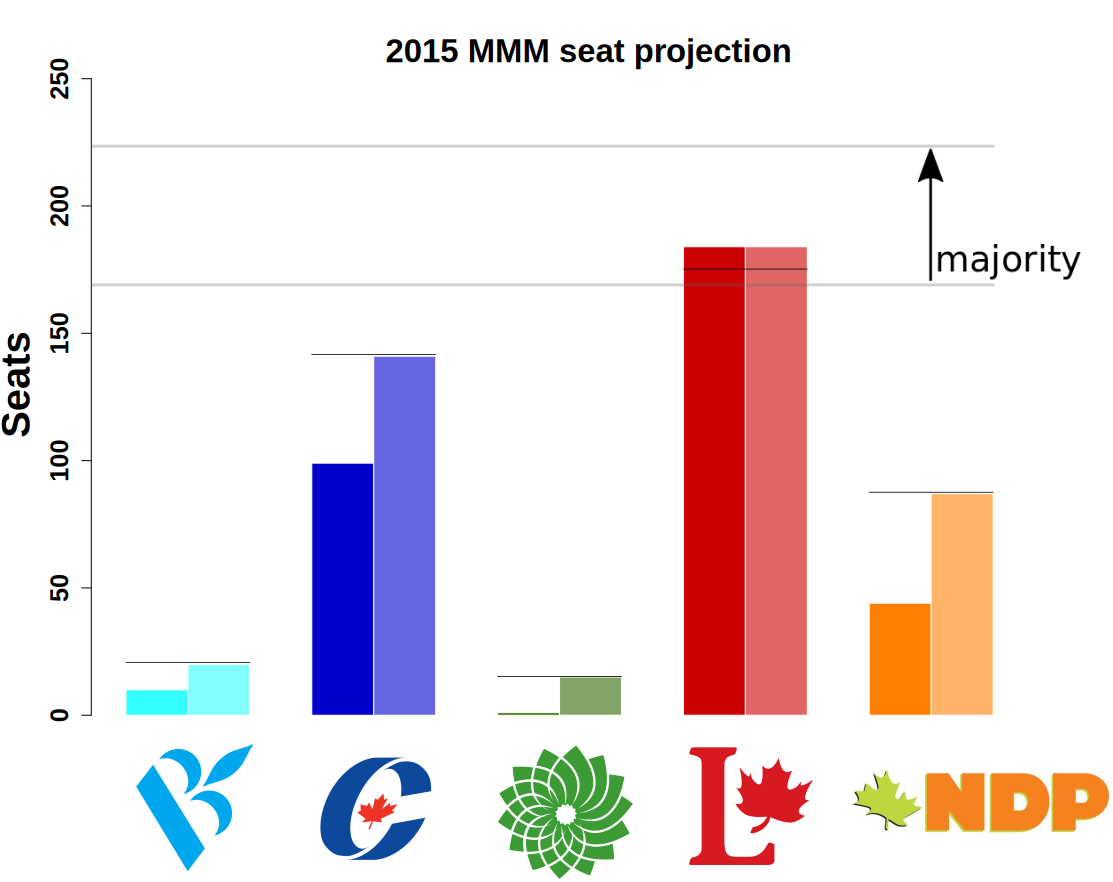
\includegraphics[width=0.50\textwidth,clip]{Figs/2015_seat_projection}
  \caption{Projected seat distribution following the 2015 federal election, using actual results (left) alongside projected results of this model from the same electorate in transparency (right). The bar defining majority control is shown in grey transparency for both cases, while a finer black line for each party shows the number of seats that would correspond to their share of the popular vote.}
\label{fig:hypo_2015_sum}
\end{figure}
